\documentclass[english,11pt, reqno, oneside]{amsart}
\usepackage{amsmath}
\usepackage{amssymb}
\usepackage[usenames,dvipsnames]{xcolor}
\usepackage[colorlinks=true,linkcolor=blue!95!black, citecolor = green!55!black,bookmarksdepth=3]{hyperref}
\usepackage{tikz}
\usetikzlibrary{calc}
\usetikzlibrary{math}
\usetikzlibrary{decorations.markings, decorations.pathreplacing,shapes.misc}

\begin{document}

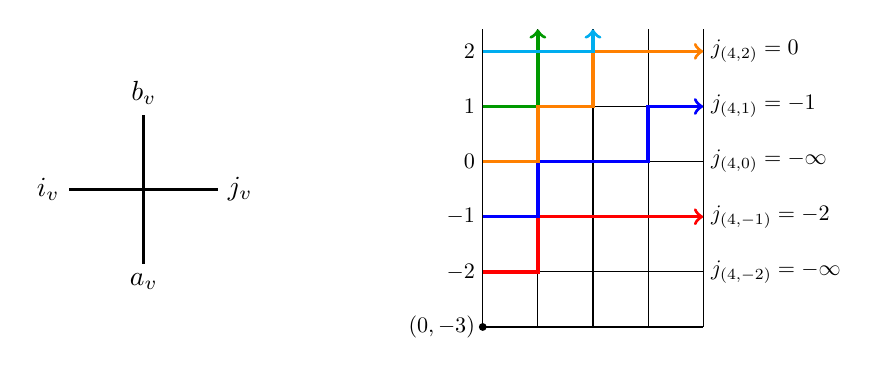
\begin{tikzpicture}[scale=0.7]

\begin{scope}[shift={(-7.5,1.5)}, scale=0.9]

\draw[line width=1pt] (0,0) -- ++(3,0);
\draw[line width=1pt] (1.5,-1.5) -- ++(0,3);

\node[anchor = east] at (0,0) {$i_v$};
\node[anchor = west] at (3,0) {$j_v$};
\node[anchor = north] at (1.5,-1.5) {$a_v$};
\node[anchor = south] at (1.5,1.5) {$b_v$};
\end{scope}

\draw (0,-1) grid (4,4.4);

\draw[red, very thick, ->] (0,0) -- ++(1,0) -- ++(0,1) -- ++(3,0);

\draw[blue, very thick, ->] (0,1) -- ++(1,0) -- ++(0,1) -- ++(2,0) -- ++(0,1) -- ++(1,0);

\draw[green!60!black, very thick, ->] (0,3) -- ++(1,0) -- ++(0,1.4);

\draw[orange, very thick, ->] (0,2) -- ++(1,0) -- ++(0,1) -- ++(1,0) -- ++(0,1) -- ++(2,0);

\draw[cyan, very thick, ->] (0,4) -- ++(2,0)-- ++(0,0.4);



\foreach \x in {-2,...,2}
{
  \node[anchor=east, scale=0.8] at (0,\x+2) {$\x$};
}

\node[circle, fill, inner sep=1pt] at (0,-1) {};
\node[anchor=east, scale=0.8] at (0,-1) {$(0,-3)$};

\node[anchor=west, scale=0.8] at (4,0) {$j_{(4,-2)}=-\infty$};
\node[anchor=west, scale=0.8] at (4,1) {$j_{(4,-1)}=-2$};
\node[anchor=west, scale=0.8] at (4,2) {$j_{(4,0)}=-\infty$};
\node[anchor=west, scale=0.8] at (4,3) {$j_{(4,1)}=-1$};
\node[anchor=west, scale=0.8] at (4,4) {$j_{(4,2)}=0$};


\end{tikzpicture}

\end{document}